\documentclass[12pt]{article}
\usepackage{amsmath}
\usepackage{graphicx}
\usepackage{enumerate}
\usepackage{natbib}
\usepackage{url} % not crucial - just used below for the URL 

%\pdfminorversion=4
% NOTE: To produce blinded version, replace "0" with "1" below.
\newcommand{\blind}{1}
\newcommand{\fulltitle}{Estimating the duration of RT-PCR positivity for SARS-CoV-2 from doubly interval censored data with undetected infections}

% DON'T change margins - should be 1 inch all around.
\addtolength{\oddsidemargin}{-.5in}%
\addtolength{\evensidemargin}{-1in}%
\addtolength{\textwidth}{1in}%
\addtolength{\textheight}{1.7in}%
\addtolength{\topmargin}{-1in}%

%% ABOVE THIS LINE IS JASA TEMPLATE
%% BELOW THIS LINE IS MY STUFF

% add bibliography to TOC - remove for final version
\usepackage[nottoc,numbib]{tocbibind}

\usepackage[utf8]{inputenc}
\usepackage{amssymb}
\usepackage{floatpag}
\usepackage{bm}
% \usepackage{algorithm2e}
\usepackage[unicode,psdextra]{hyperref}
\usepackage[nameinlink]{cleveref}
\usepackage{csquotes}
\usepackage[T1]{fontenc}
\usepackage{textcomp} % provide symbols
\usepackage{xr}
\usepackage{afterpage}
\usepackage{caption}
\usepackage{numprint}
\npfourdigitnosep
\npdecimalsign{.}
% \usepackage{microtype}
\usepackage{todonotes}

% Generic maths commands
\def\reals{\mathbb{R}}
\def\nats{\mathbb{N}}
\def\sampSpace{\mathcal{X}}
\def\dist{\sim}
\DeclareMathOperator{\E}{\mathbb{E}}
\DeclareMathOperator{\V}{\mathbb{V}}
\DeclareMathOperator{\I}{\mathbb{I}}
\DeclareMathOperator{\prob}{\mathbb{P}}
\DeclareMathOperator{\p}{\pi}
\DeclareMathOperator{\var}{\mathbb{V}}
\DeclareMathOperator{\indicator}{\mathbb{I}}
\DeclareMathOperator{\cov}{Cov}
\DeclareMathOperator{\cor}{Cor}
\DeclareMathOperator{\logit}{logit}
\DeclareMathOperator{\Ber}{Bernoulli}
\DeclareMathOperator{\Bin}{Binomial}
\DeclareMathOperator{\Poi}{Poisson}
\DeclareMathOperator{\BetaDist}{Beta}
\DeclareMathOperator{\Exponential}{Exponential}
\DeclareMathOperator{\NBr}{NegBin}
\newcommand{\NBc}{\NBr_{c}}
\newcommand{\NBs}{\NBr_{s}}
\DeclareMathOperator{\BB}{BetaBin}
\DeclareMathOperator{\GamDist}{Gamma}
\DeclareMathOperator{\MN}{Multinomial}
\DeclareMathOperator{\N}{N}
\DeclareMathOperator{\MNorm}{N}
\DeclareMathOperator{\LN}{LN}
\DeclareMathOperator{\LKJ}{LKJ}
\DeclareMathOperator{\expit}{expit}
\newcommand\matr{\bm}
\newcommand\set{\mathcal}
\renewcommand{\vec}[1]{\bm{#1}}
\newcommand{\ssep}{:}
\DeclareMathOperator*{\argmax}{arg\,max}

\newcommand\citePersonalComms[1]{(#1, personal communication)}

% Thesis-specific maths commands
\newcommand{\dmax}{d_\text{max}}
\newcommand{\psens}{p_\text{sens}}
\newcommand{\psenss}{p_\text{sens}^{(s)}}
\newcommand{\psensi}{p_\text{sens}^{(i)}}
\newcommand{\ntot}{n_\text{tot}}
\newcommand{\ndet}{n_\text{d}}
\newcommand{\nnodet}{n_\text{u}}
\newcommand{\pnodet}{p_\text{u}}
\newcommand{\Npop}{N_\text{pop}}
\newcommand{\Ncis}{N_\text{CIS}}
\newcommand{\ncis}{\vec{n_\text{CIS}}}
\newcommand{\na}{\vec{n}_\text{obs}}
\newcommand{\pcis}{\vec{p_\text{CIS}}}
\newcommand{\sched}{\mathbb{T}}
\newcommand{\nsched}{n_{\sched}}
\newcommand{\inform}{{_{\text{inform}}}}


%% Bibliography
% \usepackage[authordate-trad,backend=biber]{biblatex-chicago}
% \addbibresource{references.bib}

% Macros for common abbreviations to get the spacing right
% See: https://stackoverflow.com/questions/3282319/correct-way-to-define-macros-etc-ie-in-latex
\usepackage{xspace}
\makeatletter
\DeclareRobustCommand\onedot{\futurelet\@let@token\@onedot}
\def\@onedot{\ifx\@let@token.\else.\null\fi\xspace}
\def\eg{e.g\onedot} \def\Eg{{E.g}\onedot}
\def\ie{i.e\onedot} \def\Ie{{I.e}\onedot}
\def\cf{c.f\onedot} \def\Cf{{C.f}\onedot}
\def\etc{etc\onedot} \def\vs{{vs}\onedot}
\def\wrt{w.r.t\onedot} \def\dof{d.o.f\onedot}
\def\etal{et al\onedot}
\makeatother

%% LINE NUMBERS
% \usepackage{lineno} % Include the package for line numbering
% \linenumbers % Activates line numbering for the document

\begin{document}

%\bibliographystyle{natbib}

\def\spacingset#1{\renewcommand{\baselinestretch}%
{#1}\small\normalsize} \spacingset{1}


%%%%%%%%%%%%%%%%%%%%%%%%%%%%%%%%%%%%%%%%%%%%%%%%%%%%%%%%%%%%%%%%%%%%%%%%%%%%%%

\if1\blind
{
  \title{\bf \fulltitle}
  \author{%
    Blake, TBC, Birrell, De Angelis  
    % Author 1\thanks{
    % The authors gratefully acknowledge \textit{please remember to list all relevant funding sources in the unblinded version}}\hspace{.2cm}\\
    % Department of YYY, University of XXX\\
    % and \\
    % Author 2 \\
    % Department of ZZZ, University of WWW}
  }
  \maketitle
} \fi

\if0\blind
{
  \bigskip
  \bigskip
  \bigskip
  \begin{center}
    {\LARGE\bf \fulltitle}
\end{center}
  \medskip
} \fi

\bigskip
\begin{abstract}
The text of your abstract. 200 or fewer words.
\end{abstract}

\noindent%
{\it Keywords:}  3 to 6 keywords, that do not appear in the title
\vfill

\newpage

\listoftodos

The \textbf{format requirements from JASA} are at \url{https://www.tandfonline.com/journals/uasa20}.
\begin{itemize}
    \item Should be written with the following elements in the following order: title page; author footnote; abstract; keywords; article text (table(s); figures); acknowledgments; appendices; references
    \item Should be no more than 35 pages, including the abstract, figures, tables, and references. Appendices, proofs, and other supporting material should be placed in a separate supplement file (anonymized for review)
    \item Should contain an unstructured abstract of 200 words.
    \item Should contain between 3 and 5 keywords. Read making your article more discoverable, including information on choosing a title and search engine optimization.
    \item JASA requires that all papers be formatted for 8 1/2 x 11-inch paper, one side only.
    \item 12 point, double-spaced font (which we define as 26 lines of text per page)
    \item the average JASA paper is about 30 manuscript pages (with the above page format and including all appendices, references, tables, and figures), and it is very uncommon for papers much longer than about 35 pages to appear in JASA. 
\end{itemize}

\tableofcontents

\newpage
\spacingset{1.9} % DON'T change the spacing!
\section{Introduction} \label{sec:intro}

The duration of RT-PCR positivity is important for calculating incidence using backcalculation\todo{cite backcalc} as well as for designing public heath interventions (\eg isolation periods)\todo{cite public health use - Hellewell?}.
The duration of RT-PCR positivity for an infection episode, $j$, is (in discrete time) the number of days during an infection episode a positive RT-PCR test is returned, $D_j$.
This can be written as a function of the beginning of an infection episode (the first day the individual tests positive), $B_j$, until the end of the infection episode (the last day the individual tests positive), $E_j$, as $D_j = E_j - B_j + 1$.
It is commonly expressed as a survival function, $S_{\vec{\theta}}(d) = \prob(D_j \geq d \mid \vec{\theta})$, where $\vec{\theta}$ is a vector of parameters determining the value of $S$, and what we aim to infer.

An initial meta-analysis estimated that individuals test positive for SARS-CoV-2 for a mean of 14.6 days (95\% CI: 9.3--20.0 days)~\citep{cevikShedding}; however, most studies included in the meta-analysis involved hospitalised patients or had unclear inclusion criteria, and hence may not be representative of the general population.
This remains true of later studies~\citep[e.g.]{ealesCharacterising,hellewellPCRSensitivity}.
Furthermore, studies tend to have short follow-up and may not provide good estimates of the mean duration of positivity, which is a right-skewed distribution.
\todo{mention work on ATACCC which we'll use later}
For backcalculation, the mean is the most important feature~\citep{freemanPrevalence}, but results can be sensitive to the entire distribution.

Here, we investigate whether the Coronavirus Infection Survey (CIS)~\citep{CIS}, a longitudinal study of RT-PCR positivity in the general population, can be used to estimate the duration of positivity.
This study tested individuals at regular intervals for a long period of time (see \cref{sec:data}).
As the testing schedule was independent of infection status and had indefinite follow-up, the study provides a unique opportunity to provide an unbiased estimate of the full distribution of $D_j$ in the general population.
However, the study design uses weekly or monthly testing intervals, a design that poses several statistical challenges.

\begin{figure}
  \todo[inline]{Create figure with missing and interval censored episodes}
  \caption{%
    Challenges posed by the CIS design.
  }
  \label{fig:challenges}
\end{figure}

First, infections can be undetected.
Monthly testing is longer than many infection episodes; therefore, an infection episode could begin and end between tests (see \cref{fig:challenges}(A)).
The situation is subtly different from the standard truncation situation encountered in the literature.
In the standard situation, nothing is known about the unrecorded intervals.
But in CIS, individuals in which undetected infections occurred are enrolled in the study.
Therefore, we know the times that they were tested.
This provides information on how long their infections may have been.
We refer to these events as ``undetected'', rather than truncated, to emphasise this difference.
We address this challenge by using a Bayesian framework, and augmenting the posterior distribution with the number of undetected episodes.

Second, infection episodes are doubly interval censored.
That is, both $b_j$ and $e_j$ are only known up to an interval (see \cref{fig:challenges}(B)).
We denote the left and right intervals form $b_j$ as $l_j^{(b)}$ and $r_j^{(b)}$ respectively, and similarly for $e_j$.
Hence, $b_j \in [l_j^{(b)}, r_j^{(b)}]$ and $e_j \in [l_j^{(e)}, r_j^{(e)}]$.
We address this challenge using standard methods for doubly interval censored data.

Third, false negatives are possible.
The sensitivity of RT-PCR tests is less than 100\%~\todo{cite false negatives}, although the specificity is very high (\ie there are a negligble number of false positives)\todo{cite false positives}.
In particular, the negative test upper bounding $E_j$ could be a false negative and hence the episode lasts longer than observed.
Furthermore, this increases the number of episodes undetected.
We address this challenge by adjusting the likelihood for the sensitivity of the test.

Fourthly, short infection episodes are much more likely to be undetected.
Therefore, there is a lack of information on what proportion of episodes are short.
We address this challenge by incorporating information from a previous study as a prior distribution.

Finally, to preserve privacy, the CIS data is held in the Secure Research Service (SRS), a form of Trusted Research Environment.
The SRS contains limited computational resources\todo{describe SRS computational resources}, meaning that computationally intensive methods are infeasible.

\subsection{Related work}

\todo[inline]{This section probably needs some cuts, currently taken from my thesis directly}

Many methods exist for doubly interval censored data~\citep{sunAnalysis,bogaertsSurvival}, but few consider the additional challenges posed by undetected episodes.
Theoretical frameworks including this case exist~\citep{turnbullEmpirical,dempsterMaximum} but only the special case where the terminating event is either uncensored or right censored has been applied in practice~\citep[e.g.][]{sunEmpirical,bacchettiNonparametric,shenNonparametric}.
These studies base their inference on a likelihood contribution for each detected infection episode conditional on $b_j \in [l_j^{(b)}, r_j^{(b)}]$.

For this conditional likelihood to be valid, they assume this conditioning provides negligible information on the distribution of interest~\citePersonalComms{Nick Jewell}.
This assumption performs well in these settings, when the length of the intervals is fairly constant.
In particular, when the interval lengths are near-constant, $p(\text{episode $j$ detected} \mid b_j \in [l_j^{(b)}, r_j^{(b)}]) \approx p(\text{episode $j$ detected})$.
However, the interval lengths change from one to four weeks in the CIS.

Infection episodes in an individual's one-week testing period are over-represented in the detected infections.
This is because more frequent testing will detect a higher proportion of infections.
Therefore, for the average detected episode, $p(\text{episode $j$ detected} \mid b_j \in [l_j^{(b)}, r_j^{(b)}]) > p(\text{episode $j$ detected})$ and conditioning on $b_j \in [l_j^{(b)}, r_j^{(b)}]$ is inappropriate.

Alternative approaches exist for assessing the survival time of bird and insect nests~\citep{heiseyABCs,heiseyModelling}.
Here though, the visit times (possible detection times) are common to all the individuals, simplifying the likelihood.

The inclusion of false negatives into survival analysis is an area of much interest, especially in the application of tests for HIV in infants~\citep[e.g.][]{brownBayesian,balasubramanianEstimation};
\citet{piresIntervalMisclassify} provide a comprehensive review of approaches.
However, including false negatives with either doubly censored or truncated data has not been addressed.
The situation here requires both.

\subsection{Paper structure}

\todo[inline]{Explain the paper structure once the paper is written}
\todo[inline]{Link to code and packages}


\section{Study design and data} \label{sec:data}

The CIS~\citep{CIS} was set up in April 2020.
The dataset is globally unique in providing a representative, longitudinal, and large-scale study across the pandemic.
% Initially, it was limited to England, but expanded to cover the whole of the UK in September 2020.
Enrolment was continuous until 31st Jan 2022, with data collected until 13th Mar 2023~\citep{weiRisk}. 

We focus on the period between 10 Oct 2020 and 6 Dec 2020 inclusive, denoted as $1, \dots, T$.
This period has fairly stable prevalence, as measured by the CIS\todo{cite stable prevalence}, reducing the impact of epidemic phase bias\todo{cite epidemic phase bias}.
Additionally, it is prior to either vaccination or the emergence of the alpha variant, which likely impact the duration of RT-PCR positivity\todo{cite alpha variant impact}.
Our analysis considers the cohort of $\Ncis = \numprint{437590}$ individuals with at least one test in the interval $[1, T]$.
We index these individuals by $i = 1, \dots, \Ncis$.

The CIS had a household-based design inviting all individuals aged 2 and over from selected households.
Once invited, an enrolment swab would be taken at the first visit followed by 4 further weekly visits (giving a total of 5 swabs on days 0, 7, 14, 21, 28 relative to enrolment) after which visits were monthly.
Swabs were tested for the presence of SARS-CoV-2 using RT-PCR.
In reality, visits were often not on this precise schedule, and occasionally missed (\eg a test would occur on days 28 and 84 but not 56).
A full description of the study can be found in the study protocol~\citep{cisProtocol}.

We denote by $\sched_i$ the set of times individual $i$ is tested at, starting from their last test prior to time 1, if it exists, or their first test following enrolment in the study otherwise; note that $\sched_i$ includes any tests that occur after $T$.
Each individual has exactly one test schedule, but it is possible that $\sched_i = \sched_{i'}$ for $i \neq i'$.
We assume that the test schedules are uninformative on all quantities of interest because they are part of the study design.
Therefore, we condition on them implicitly in all probabilities that follow.


\todo[inline]{Perhaps the following paragraph is too repetitive: the notation is already defined, although it is important to relate it to the observations}
Positive tests are grouped into infection episodes~\citep{weiRisk}.
In addition, an infection episode can contain \emph{intermittent negatives}, which are false negative tests occurring between positive tests for the same infection episode.
The crucial features of an infection episode are the start and end times of the infection.
Ignoring misclassified test results, latent start time of infection episode $j$, $B_j$, can be bounded as between the day after the last negative test, $l_j^{(b)}$, and the day of the first positive test, $r_j^{(b)}$.
Similarly, the latent end time of infection episode $i$, $E_j$, can be bounded as between the day of the last positive test, $l_j^{(e)}$, and the day before the following negative test, $r_j^{(e)}$.
The information about $j$ is fully contained in the vector $o_j = [l_j^{(b)}, r_j^{(b)}, l_j^{(e)}, r_j^{(e)}, i_j]^T$ where $i_j$ is the individual episode $j$ occurred in.

We analyse the $\ndet = \numprint{4800}$ episodes satisfying the following inclusion criteria.
\begin{enumerate}
  \item The episode's first positive test occurred between 10 Oct 2020 and 6 Dec 2020 inclusive, \ie $r_j^{(b)} \in [1, T]$.
  \item A negative test bounds both the beginning and end of the episode, meaning both $l_j^{(b)}$ and $r_j^{(e)}$ exist.
\end{enumerate}
There are $\ndet = \numprint{4800}$ such episodes.



\section{Inference framework} \label{sec:inference}

We start by developing a computationally feasible Bayesian statistical model accounting for double interval censoring and undetected episodes, assuming that there are no misclassified test results.
A Bayesian framework provides uncertainty quantification, which is otherwise challenging in this setting~\citep{sunAnalysis,dengNonparametric}.
Additionally, it allows for the incorporation of prior information which helps overcome the challenges posed by undetected episodes~\citep{caoBias}.

\todo[inline]{Perhaps there should be a sentence or two here about the structure of the section}

The target of inference is $\vec{\theta}$, the parameters of the survival function $S_{\vec{\theta}}(t) = \prob(D_j \geq t \mid \vec\theta)$; its composition is discussed in \cref{sec:parameters-priors}.

We augment the posterior distribution with the total number of infection episodes, $\ntot = \ndet + \nnodet$, where $\nnodet$ is the number of undetected infection episodes that occurred in one of the $\Ncis$ individuals; $\nnodet$ is latent.
Infection episodes are indexed by $j = 1, \dots, \ntot$.
If $j$ is a detected episode, then $o_j = [l_j^{(b)}, r_j^{(b)}, l_j^{(e)}, r_j^{(e)}, i_j]^T$, as before.
If $j$ is undetected, then define $o_j = \emptyset$.

The observation $o_j$ is a realisation of the discrete random variable $O_j$.
Define $O_j$'s state space as $\set{E}' = \{ \emptyset \} \cup \set{E}$ where $\set{E} = \{ \vec{\nu}_1, \dots, \vec{\nu}_{N_E} \}$ is the set of all $N_E$ (a priori) possible unique observations of detected episodes.
Therefore, $\vec{\nu}_k = [l^{(b)}_k, r^{(b)}_k, l^{(e)}_k, r^{(e)}_k, i_k]^T$ for $k = 1, \dots, N_E$.

Let $p_k = \prob(O_j = \vec{\nu}_k \mid \vec{\theta})$, the probability that $O_j$ takes the value $\vec{\nu}_k$.
Similarly, let $p_u = \prob(O_j = \emptyset \mid \vec{\theta})$, the probability that $j$ is undetected.
Then, the probability distribution for $O_j$ is specified by $\vec{p} = [p_1, \dots, p_{N_E}, p_u]^T$.

Let $n_k$ denote the number of times $\vec{\nu}_k$ is observed; $\nnodet$ denote the latent number of undetected episodes; and $\vec{n} = [n_1, \dots, n_{N_E}, \nnodet]^T$.
Formally, $n_k = \sum_{j=1}^{\ntot} \indicator(O_j = \vec{\nu}_k)$ and $\nnodet = \sum_{j=1}^{\ntot} \indicator(O_j = \emptyset)$.
Hence, $\ndet = \sum_{k=1}^{N_E} n_k$.
Assume, for tractability, that the events $O_j = \vec{\nu}_k$ and $O_{j'} = \vec{\nu}_{k'}$ are independent for $j \neq j'$ (conditional on $\theta$); this assumption is discussed in \cref{sec:discussion}.
Hence:
\begin{align}
  \vec{n} \mid \ntot, \vec{\theta} &\dist \MN(\ntot, \vec{p})
\intertext{that is:}
  p(\vec{n} \mid \ntot, \vec{\theta}) &= \frac{\ntot!}{\nnodet!\prod_{k=1}^{N_D} n_k!} p_u^{\nnodet} \prod_{k=1}^{N_D} p_k^{n_k}.
  \label{perf-test:eq:multinomial-ll}
\end{align}
\begin{figure}
\makebox[\textwidth][c]{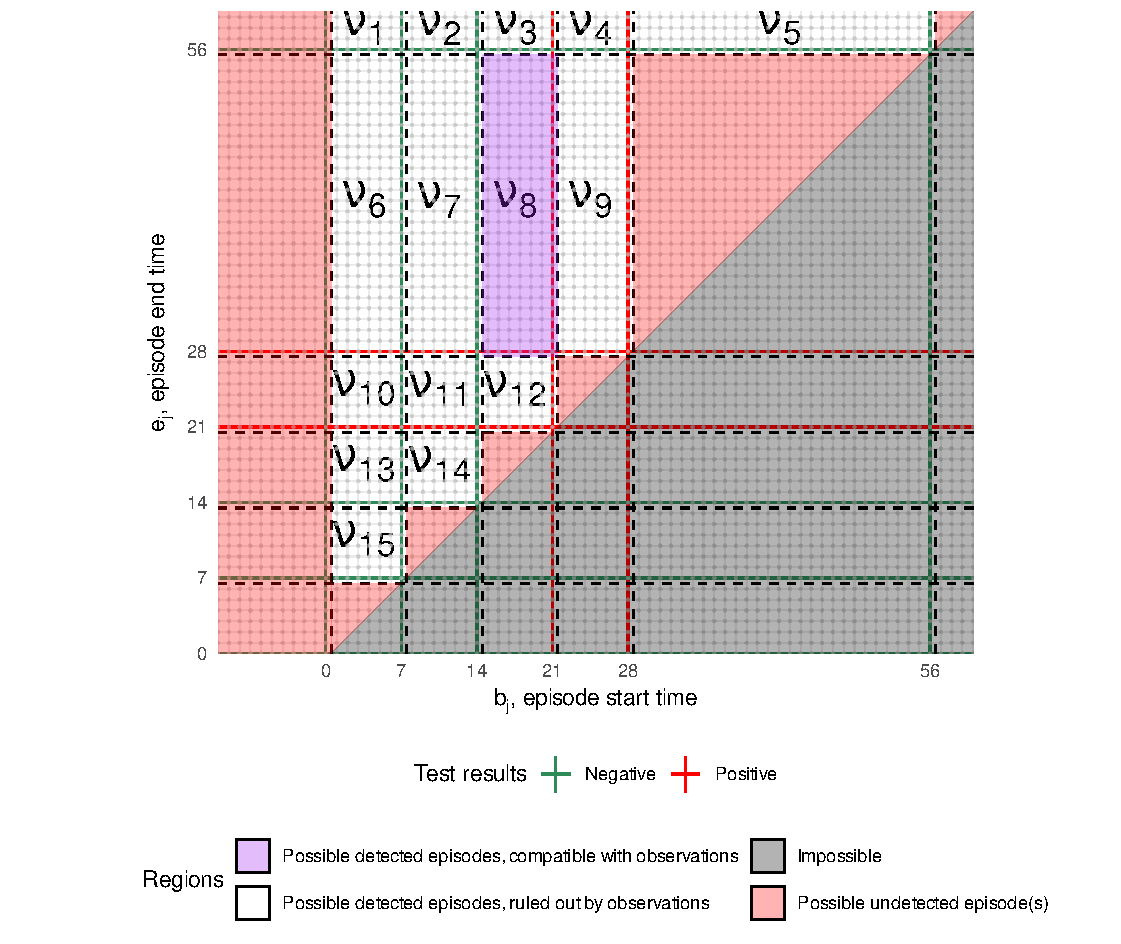
\includegraphics[width=0.9\paperwidth]{figures/output/regions_diag}}
\thisfloatpagestyle{empty}
\caption[Episode regions]{%
  Each dot is a combination of $b_j$ and $e_j$ for an arbitrary individual $i$.
  The combinations giving rise to the same value of $\nu_k$ are in the same box, bounded by dashed lines.
  $i$ had negative tests at times 0, 7, 14, 56, and 84 (not shown) and positive tests at times 21 and 28.
  The purple region corresponds to the doubly interval censored episode in this individual.
  That is, $n_8 = 1$ and $n_k = 0$ for $k = 1, \dots, 7, 9, \dots, 15$.
  The red region corresponds to combinations giving $O_j = \emptyset$.
  Impossible region violates $b_j \leq e_j$.
}
\label{perf-test:fig:partitionSpace}
\end{figure}

In the CIS data, each $n_k$ ($k \neq u$) is observed as either 0 or 1.
Define $\set{D} = \{ k \ssep n_k = 1 \}$, the detected episodes.
Furthermore, note that the support of the multinomial distribution requires that $\nnodet = \ntot - \ndet$.
Let $\na = [n_{1}, \dots, n_{N_E}]^T$ be the observed portion of $\vec{n}$.
Then \cref{perf-test:eq:multinomial-ll} simplifies to:
\begin{align}
  p(\vec{n} \mid \ntot, \vec{\theta})
  &= p(\na \mid \ntot, \vec{\theta}) \\
  &= \frac{\ntot!}{(\ntot - \ndet)!} p_u^{\ntot-\ndet} \prod_{k \in \set{D}} p_k.
  \label{perf-test:eq:multinomial}
\end{align}

The relevant information from the CIS data is fully contained in the vector $\na$.
Therefore, the posterior of interest is (see\todo{ref appendix} for the full derivation):
\begin{align}
p(\vec{\theta} \mid \na)
&\propto  p(\vec{\theta}) \left( \prod_{k \in \set{D}} p_k \right) \left( \sum_{\ntot=\ndet}^\infty p(\ntot \mid \vec{\theta}) \frac{\ntot!}{(\ntot - \ndet)!} \pnodet^{\ntot - \ndet} \right).
\label{perf-test:eq:posterior1}
\end{align}

For mathematical convenience, we assume the prior $\ntot \dist \NBc(\mu, r)$, and that it is independent of $\vec{\theta}$, the parameters of the survival distribution.
In this case \cref{perf-test:eq:posterior1} simplifies to (see\todo{cite appropriate appendix}):
\begin{align}
p(\vec{\theta} \mid \na)
&\propto p(\vec{\theta}) \left( \prod_{i \in \set{D}} p_k \right) (r + \mu (1- \pnodet))^{-(r+\ndet)} \label{perf-test:eq:full-posterior}.
\end{align}

The rest of this section derives expressions for each of $p_{k}$, $p_{u}$ and $\eta$.

Decompose $p_k$ as $p_k = p_{ik} \prob(i_j = i_k \mid \vec{\theta})$
where $p_{ik} = \prob(O_j = \vec{\nu}_k \mid i_j = i_k, \vec{\theta})$.
% This is valid as $\prob(O_j = \nu_k \mid i_j \neq i_k) = 0$ due to the condition here being equivalent to equating the two vectors' final elements.
Assume that each infection episode occurs independently and with equal probability in any individual, \ie $\prob(i_j = i_k) = 1/\Ncis$ for all $j$ and $k$, and $B_j$ takes values with uniform probability from its state space.

Therefore, $p_{ik}$ takes the standard form of the likelihood for doubly interval censored data without truncation (see\todo{ref appendix} for details):
\begin{align}
p_{ik}
\propto& \sum_{b = l_k^{(b)}}^{r_k^{(b)}} \left( S_{\vec{\theta}}(l_k^{(e)} - b + 1) - S_{\vec{\theta}}(r_k^{(e)} - b + 2) \right).
\label{perf-test:eq:pia}
\end{align}

The remaining component of \cref{perf-test:eq:full-posterior} required is $1- p_u$, one minus the probability of missing an infection, \ie the probability of detecting an infection.

\subsection{Deriving $1 - p_u$} \label{sec:prob-undetected}

The final component of \cref{perf-test:eq:full-posterior} required is $1 - p_u$.
Recall the definition $p_u = \prob(O_j = \emptyset \mid \vec{\theta})$.
Therefore:
\begin{align}
  1 - p_u
  &= 1 - \sum_{i=1}^{\Ncis} \prob(O_j = \emptyset, i_j = i \mid \vec{\theta}) \\
  &= 1 - \sum_{i=1}^{\Ncis} \prob(O_j = \emptyset \mid i_j = i, \vec{\theta}) P(i_j = i \mid \vec{\theta}) \\
  &= 1 - \frac{1}{\Ncis}\sum_{i=1}^{\Ncis} \prob(O_j = \emptyset \mid i_j = i, \vec{\theta}) \\
  &= \frac{1}{\Ncis} \sum_{i=1}^{\Ncis} (1 - \prob(O_j = \emptyset \mid i_j = i, \vec{\theta}))
  \label{perf-test:eq:pu}
\end{align}
assuming $P(i_j = i \mid \vec{\theta}) = 1/\Ncis$ as before.
Let $p_{iu} = \prob(O_j = \emptyset \mid i_j = i, \vec{\theta})$.
Therefore, the crucial component is $1 - p_{iu}$.
This is one minus the probability that an episode in individual $i$ was undetected, \ie the probability of the episode being detected.

An episode $j$ in individual $i_j$ is detected if and only if all the following conditions are met.
\begin{enumerate}
    \item $\exists t \in \sched_{i_j}$ such that $b_j \leq t \leq e_j$; this condition is equivalent to having at least one positive test for the episode.
    \item $b_j > \min \sched_{i_j}$.
      For individuals enrolled during the period considered ($\min \sched_{i_j} > 0$), this ensures that the beginning of the episode is lower bounded; thereby adjusting for those who enrolled during the period being less likely to have a detected infection.
      For individuals enrolled prior to the period considered ($\min \sched_{i_j} \leq 0$), this means that the episode was not detected prior to time 1.
    \item $b_j \leq T_{i_j}$ where $T_{i_j} = \max \{ t \in \sched_{i_j} \ssep t \leq T \}$ is the last time that $i_j$ is tested in the period, meaning that the test is detected within the period.
    \item $\exists t \in \sched_{i_j}$ such that $t > e_j$, upper bounding the end of the episode.
      For episodes detected in the period we consider, a negligible number of episodes are excluded due to this critera.
      It only occurs in individuals lost to follow-up; therefore, we neglect this possibility.
      % For a new context, including recent infections, this condition could be relaxed by considering episodes that do not meet this criterion as right censored.
\end{enumerate}

% An episode is undetected if and only if no tests are performed during the episode or if there was no negative test prior to the episode.
% Equivalently, that the first test at or after $b$ is after $e$, or that there is no negative test prior to $b$.
First define $\tau_{\sched_i}(t)$ as the time until the next test at or after time $t$ in the schedule $\sched_i$:
\begin{align}
\tau_{\sched_i}(t) &= \min \{ t' \in \sched_i : t' \geq t \} - t
\label{perf-test:eq:tau-def}
\end{align}
% defining $\min \emptyset = \infty$; \ie $\tau_{\sched_i}(t) = \infty$ if there is no $t' \in \sched_i$ such that $t' \geq t$.
The first condition can now be expressed as $e_j \geq b_j + \tau_{\sched_{i_j}}(b_j)$.
Equivalently, $d_j \geq \tau_{\sched_{i_j}}(b_j) + 1$.
% The fourth condition can be expressed as $\tau_{\sched_{i_j}}(b_j) < \infty$.


% Then $\Omega_i$ can be written as:
% \begin{align}
% \Omega_i = \{ (b, e) \ssep \tau_{\sched_i}(b) + b > e \vee b \leq \min(\sched_i) \}.
% \end{align}
Therefore, omitting the conditioning on $\vec{\theta}$ and $i_j = i$:
\begin{align}
1 - p_{iu}
% &= 1 - \prob((B_{j}, E_{j}) \in \Omega_i) \\
&= \prob(D_j \geq \tau_{\sched_{i}}(B_j)+ 1, \min \sched_{i_j} < B_j \leq T_{i_j}) \\
&= \sum_{b = \min \sched_{i} + 1}^{T_{i_j}} \prob(D_j \geq \tau_{\sched_{i}}(b) + 1 \mid B_j = b) \prob(B_j = b)\\
&\propto \sum_{b = \min \sched_{i} + 1}^{T_{i_j}} S_{\vec{\theta}}(\tau_{\sched_{i}}(b) + 1).
\label{perf-test:eq:piu}
\end{align}

Substituting into \cref{perf-test:eq:pu}:
\begin{align}
1 - p_u
& \propto \sum_{i=1}^{\Ncis} \sum_{b = \min \sched_{i} + 1}^{T_{i_j}} S_{\vec{\theta}}(\tau_{\sched_{i}}(b) + 1).
\end{align}

\section{Handling false negatives} \label{sec:false-negatives}

Now we modify the survival framework to incorporate false negatives (\ie allowing $\psens < 1$).
Using a simple model, in particular a constant test sensitivity, means calculating the likelihood remains tractable.

We start, in \cref{imperf-test:sec:notation}, by introducing some additional notation needed.
We then modify the components of the likelihood in \cref{imperf-test:sec:modifying-p_ia,imperf-test:sec:modifying-p_iu} to incorporate false negatives.


\subsection{Notation} \label{imperf-test:sec:notation}

Introducing false negatives means that $O_j$, the observation vector of episode $j$, is now random, even if $B_j$ and $E_j$ are known.
Therefore, the results between the tests that bound episode $j$'s beginning and end times should now enter into the likelihood.
For tractability, we include only tests between the negative tests at $l_j^{(b)}-1$ and $r_j^{(e)}+1$. 

To formalise this, we define analogous variables to those in \cref{sec:inference}.
To start with, define the relevant testing times for any episode $j$ with $O_j = \vec{\nu}_k$ as $\sched'_k = \{ t \in \sched_{i_k} \ssep r_k^{(b)} \leq t \leq r_k^{(e)} + 1 \}$ and let $m_k$ denote the size of this set.
Denote the elements of $\sched'_k$ by $t_{k,1} < \dots < t_{k,m_k}$.
Let $\set{E}' = \{ \vec{\nu}_1', \dots, \vec{\nu}_{N_E'}' \}$ be a new set of possible observations of detected episodes, including the pattern of positive and negative tests.
Represent the observations such that for any $\vec{\nu}_k' \in \set{E}'$, $\vec{\nu}_k' = [\vec{\nu}_{k}, \vec{y}_k]^T$, where $\vec{y}_k \in \{ 0, 1 \}^{m_k}$ with $y_{k,l}$ being the test result at time $t_{k,l}$.

$\vec{\nu}'_k \in \set{E}'$ occurs if and only if all the following conditions are met.
\begin{enumerate}
  \item $\vec{\nu}_k \in \set{E}$.
  \item The elements of $\vec{y}_k$ corresponding to the tests at times $r_k^{(b)}$ and $l_k^{(e)}$ are positive, \ie $y_{k,1} = y_{k,m_k-1} = 1$.
  \item The element of $\vec{y}_k$ corresponding to the test at time $r_k^{(e)} + 1$ is negative, \ie $y_{k,m_k} = 0$.
\end{enumerate}
The final two conditions are due to the construction of the intervals as positive and negative tests bounding the beginning and end times of the episode.
As condition 2 requires $y_{k,1} = 1$ and condition 3 requires $y_{k,m_k} = 0$, these conditions can only occur if $m_k \neq 0$.
Therefore, $m_k \geq 2$.

Let $O'(j)$ be the observations generated by episode $j$ including the new vector of results.
As before, $O'(j) \in \set{E}'$ indicates that episode $j$ was detected; otherwise, $O'(j) = \emptyset$.

Similarly, we define $p_k'$, $p_{ik}'$, $p_u'$, and $p_{iu}'$ to replace $p_k'$, $p_{ik}'$, $p_u'$, and $p_{iu}'$ respectively.
\begin{align}
    p_{ik}' &= \prob(O'(j) = \vec{\nu}'_k \mid i_j = i_k, \vec{\theta}) \\
    p_k' &= \frac{1}{\Ncis} p_{ik}' \\
    p_{iu}' &= \prob(O'(j) = \emptyset \mid i_j = i_k, \vec{\theta}) \\
    p_u' &= \frac{1}{\Ncis} \sum_{i=1}^{\Ncis} p_{iu}'.
\end{align}

\subsection{Deriving $p'_{ik}$} \label{imperf-test:sec:modifying-p_ia}

We will modify $p_{ik}$ to form $p_{ik}' = \prob(O'(j) = \vec{\nu}'_k \mid i_j = i_k, \vec{\theta})$, taking into account false negatives.
We consider a mixture of two scenarios, whether the final test in $\sched'_{k}$ is a false negative, with the mixture probability determined by the test sensitivity.

Similar likelihoods have previously appeared in the literature~\citep[e.g.][eq.\ (2)]{piresIntervalMisclassify}.
However, this prior work was for singly interval censored data; incorporating the double interval censored nature of the CIS data involves summing over the possible episode start times.

% We proceed by assuming that we have observed an arbitrary episode:
% \begin{align}
%   O'(j) = [[l_k^{(b)}, r_k^{(b)}, l_k^{(e)}, r_k^{(e)}, i_j]^T, \vec{y}_k]^T.
% \end{align}
% We derive $p_k$ by considering the generating process that could have produced this episode.

For tractability, assume that the negative test bounding the start of the episode, on day $l_k^{(b)}-1$, is a true negative.
This assumption is reasonable because, since a positive test follows at $r_k^{(b)}$, the negative at $l_k^{(b)}-1$ is likely early in the infection and the test sensitivity is high early in an infection.
True negatives occur with probability 1, and hence this test does not contribute to the likelihood.

As we assume that there are no false positives, the infection episode must span at least the period $[r^{(b)}_k, l^{(e)}_k]$, a period starting and ending with a positive test.
This includes all $t \in \sched'_k$ except $t = r_k^{(e)}+1$.
Therefore, the test results $\vec{y}_k$, except the test at $r_k^{(e)}+1$, are either true positives or false negatives.
This gives $t_+ = \sum_{l=1}^{m_k-1} y_{k,l}(t)$ true positives and $f_- = \sum_{l=1}^{m_k-1} (1 - y_{k,l}(t))$ false negatives.

Consider the negative test at $r_k^{(e)}+1$, the first negative after the start of the episode which may be either a true or false negative.
It is a false negative if and only if the episode ends at or after the test, \ie $E_j > r_k^{(e)}$.
We proceed by first considering whether this is the case and conditioning on $B_j = b$.
Then, we combine the cases and remove the conditioning.

First, the case when $E_j \leq r_k^{(e)}$.
In this case, the test at $r_k^{(e)}+1$ is a true negative and the end of the episode is interval censored as in the previous chapter.
% In this case, the test at $r_k^{(e)} + 1$ is a true negative, as are all other tests not in $\sched'_{k}$.
The true negative occurs with probability 1, by the assumption of no false positives.
\begin{align}
&\prob(O'(j) = \vec{\nu}_k', E_j \leq r_k^{(e)} \mid B_j = b, i_j = i_k, \psens, \vec{\theta}) \\
&= \prob(O'(j) = \vec{\nu}_k', l_k^{(e)} \leq E_j \leq r_k^{(e)} \mid B_j = b, i_j = i_k, \psens, \vec{\theta}) &\text{the test at $l_k^{(e)}$ is positive} \\
&= \prob(O'(j) = \vec{\nu}_k' \mid l_k^{(e)} \leq E_j \leq r_k^{(e)}, B_j = b, i_j = i_k, \psens, \vec{\theta}) \\
&\ \ \  \times \prob(l_k^{(e)} \leq E_j \leq r_k^{(e)} \mid B_j = b, i_j = i_k, \psens, \vec{\theta}) \\
&= p_\text{sens}^{t_+} (1 - p_\text{sens})^{f_-} \left( S_{\vec{\theta}}(l_k^{(e)} - b + 1) - S_{\vec{\theta}}(r_k^{(e)} - b + 2) \right)
\label{imperf-test:eq:ll-ei-lt-ri}
\end{align}

Second, the case when $E_j > r_k^{(e)}$.
In this case, the test at $r_k^{(e)}+1$ is a false negative, occurring with probability $(1 - p_\text{sens})$.
To avoid having to consider tests after $r_k^{(e)}$, which could greatly complicate the likelihood, we model this case as the episode being right censored at $r_k^{(e)}$.
Taking the same approach as before:
\begin{align}
&\prob(O'(j) = \vec{\nu}_k', E_j > r_k^{(e)} \mid B_j = b, i_j = i_k, \psens, \vec{\theta}) \\
&= \prob(O'(j) = \vec{\nu}_k' \mid E_j > r_k^{(e)}, B_j = b, i_j = i_k, \psens, \vec{\theta}) \\
  &\ \ \  \times \prob(E_j > r_k^{(e)} \mid B_j = b, i_j = i_k, \psens, \vec{\theta}) \\
&= p_\text{sens}^{t_+} (1 - p_\text{sens})^{f_-} (1 - p_\text{sens}) S_{\vec{\theta}}(r_k^{(e)} - b + 2)
\label{imperf-test:eq:ll-ei-gt-ri}
\end{align}

These expressions can now be used to derive $p'_{ik}$.
First, augment the data with $b$, and split into the cases just discussed, omitting the conditioning on $\psens$, $\vec{\theta}$, and $i_j = i_k$:
\begin{align}
p_{ik}'
=& \prob(O'(j) = \vec{\nu}_k') \\
=& \sum_{b = l_k^{(b)}}^{r_k^{(b)}} \left( \prob(O'(j) = \vec{\nu}_k', E_j \leq r_k^{(e)} \mid B_j = b) + \prob(O'(j) = \vec{\nu}_k, E_j > r_k^{(e)} \mid B_j = b) \right) \prob(B_j = b). \\
\intertext{Now, substitute in \cref{imperf-test:eq:ll-ei-lt-ri,imperf-test:eq:ll-ei-gt-ri} and take out the common factor:}
=\ &  p_\text{sens}^{t_+} (1 - p_\text{sens})^{f_-} \\
 & \times \sum_{b = l_k^{(b)}}^{r_k^{(b)}} \left( S_{\vec{\theta}}(l_k^{(e)} - b + 1) - S_{\vec{\theta}}(r_k^{(e)} - b + 2) + (1 - p_\text{sens}) S_{\vec{\theta}}(r_k^{(e)} - b + 2) \right) \\ 
  & \times \prob(B_j = b \mid p_\text{sens}, \vec{\theta}) \\
=\ &  p_\text{sens}^{t_+} (1 - p_\text{sens})^{f_-} \\
  & \times \sum_{b = l_k^{(b)}}^{r_k^{(b)}} \left( S_{\vec{\theta}}(l_k^{(e)} - b + 1) - p_\text{sens} S_{\vec{\theta}}(r_k^{(e)} - b + 2) \right) \\
  & \times \prob(B_j = b \mid p_\text{sens}, \vec{\theta}).
\label{imperf-test:eq:pia-prime}
\end{align}
Note that if $p_\text{sens} = 1$ then $p_{ik}' = p_{ik}$ (see \cref{perf-test:eq:pia}).

If $\psens$ is fixed (\ie has a point prior) and $\prob(B_j = b \mid \psens, \vec{\theta}) \propto 1$ then:
\begin{align}
p_{ik}'
&\propto \sum_{b = l_k^{(b)}}^{r_k^{(b)}} S_{\vec{\theta}}(l_k^{(e)} - b + 1) - p_\text{sens} S_{\vec{\theta}}(r_k^{(e)} - b + 2).
\label{imperf-test:eq:pia-prime-constant}
\end{align}

\subsection{Deriving $p'_{iu}$} \label{imperf-test:sec:modifying-p_iu}

We now modify $p_{iu}$ to form $p_{iu}' = \prob(O'(j) = \emptyset \mid i_j = i, \vec{\theta})$ to take into account false negatives.
Several mechanisms for episodes being undetected were previously considered when deriving $p_{iu}$, we now consider the additional mechanisms arising due to false negatives.
Specifically, episode $j$ could be undetected if the first test after $b_j$ is a false negative and then there are no subsequent positive tests.

This false negative would occur at the first test after the infection episode begins, on day $b_j + \tau_{\sched_{i_j}}(b_j)$.
A false negative occurring requires that the episode has not yet ended but a negative still occurs.
The episode has not yet ended at the time of the test if $e_j = b_j + d_j - 1 \geq b_j + \tau_{\sched_{i_j}}(b_j)$, that is the duration of the infection $d_j \geq \tau_{\sched_{i_j}}(b_j) + 1$.
Conditional on the episode having not yet ended, the test result is negative with probability $1 - \psens$.

For there to be no subsequent positive tests, all tests up until day $e_j$ are false negatives.
We assume there is a negligible probability of missing an episode due to two false negative tests.
This is because that would require both a long episode, encompassing two test times, and for both these tests to be false negatives.
Therefore, an episode is undetected only if the episode ends before a second test.
Denote the number of days between $b_j$ and the test following the false negative as $\tau^2_{\sched_{i_j}}(b_j) \stackrel{\text{def}}{=} \tau_{\sched_{i_j}}(\tau_{\sched_{i_j}}(b_j) + 1)$.
Then, the episode ends before this test if $d_j \leq \tau^2_{\sched_{i_j}}(b_j)$.

Therefore, this mechanism causes episode $j$ to be undetected if all the following conditions hold.
\begin{enumerate}
    \item The episode would have been detected considering only the mechanisms in \cref{sec:prob-undetected}. That is $\min(\sched_{i_j}) < b_j \leq T_{i_j}$ and $e_j \geq \tau_{\sched_{i_j}}(b_j) + b_j$.
    \item The episode ends in the interval $[\tau_{\sched_{i_j}}(b_j) + b_j, \tau^2_{\sched_{i_j}}(b_j) + b_j - 1]$.
      Note that the lower bound here is exactly the bound on $e_j$ in the previous condition.
      Equivalently, $\tau_{\sched_{i_j}}(b_j) + 1 \leq d_j \leq \tau^2_{\sched_{i_j}}(b_j)$.
    \item A false negative occurs on day $\tau_{\sched_{i_j}}(b_j) + b_j$. Conditional on the previous condition, this occurs with probability $1 - \psens$.
\end{enumerate}

The probability of this occurring, conditional on $B_j = b$ where $\min(\sched_{i_j}) < b \leq T_{i_j}$ is:
\begin{align}
&\prob \left(
    \tau_{\sched_{i_j}}(b) + 1 \leq D_j \leq \tau^2_{\sched_{i_j}}(b)
    \mid B_j = b, \vec{\theta} \right) (1 - \psens) \\
&= \left( S_{\vec{\theta}}(\tau_{\sched_{i_j}}(b) + 1) - S_{\vec{\theta}}(\tau^2_{\sched_{i_j}}(b) + 1) \right) (1 - \psens).
\end{align}
Summing over $b$, in the same way as \cref{perf-test:eq:piu}, gives:
\begin{align}
\zeta = (1 - p_\text{sens})\frac{1}{T} \sum_{b=\min(\sched_{i_j}) + 1}^{T_{i_j}} \left( S_{\vec{\theta}}(\tau_{\sched_{i_j}}(b) + 1) - S_{\vec{\theta}}(\tau^2_{\sched_{i_j}}(b) + 1) \right).
\label{imperf-test:eq:zeta}
\end{align}

$p_{iu}'$ is the probability of episode $i$ being undetected, considering both the previous and new mechanisms.
The previous and new mechanisms are mutually exclusive.
Hence, $p_{iu}'$ is the sum of these, $p_{iu}' = p_{iu} + \zeta$.
As previously, $1 - p_{iu}'$ is the required quantity.
\begin{align}
1 - p_{iu}'
=& 1 - p_{iu} - \zeta \\
=& \frac{1}{T} \sum_{b = \min \sched_{i} + 1}^{T_{i_j}} S_{\vec{\theta}}(\tau_{\sched_{i}}(b) + 1) \\
&- (1 - p_\text{sens})\frac{1}{T} \sum_{b=\min(\sched_{i_j}) + 1}^{T_{i_j}} \left( S_{\vec{\theta}}(\tau_{\sched_{i_j}}(b) + 1) - S_{\vec{\theta}}(\tau^2_{\sched_{i_j}}(b) + 1) \right) \\
=& \frac{1}{T} \sum_{b=\min(\sched_{i_j}) + 1}^{T_{i_j}} \left( p_\text{sens} S_{\vec{\theta}}(\tau_{\sched_{i_j}}(b) + 1) + (1 - p_\text{sens}) S_{\vec{\theta}}(\tau^2_{\sched_{i_j}}(b) + 1)\right).
\label{imperf-test:eq:pit-prime}
\end{align}


\section{The survival function} \label{sec:parameters-priors}

Next we specify the form and priors for $S_{\vec{\theta}}(t)$.
We parameterize $S$ in terms of the hazard $S_{\vec{\theta}}(t) = \prod_{i=1}^{t-1} (1 - \lambda_{i})$; the lack of monotonicity or sum constraint on the hazard makes it an attractive parameterization for inference~\citep{heBayesian}.
Therefore, $\vec{\theta} = [\lambda_1, \dots, \lambda_{\dmax-1}]^T$.

We consider two priors.
The first is vague for $S$, although informative on $\lambda$.
The second is informative, incorporating prior information

\subsection{Vague prior} \label{sec:vague-prior}

First, we consider independent priors on each parameter.
Each hazard, $\lambda_t$, is a (conditional) probability, and hence a Beta distribution is a natural choice.

Uninformative Beta priors, of the form $\lambda_t \dist \BetaDist(\alpha, \alpha)$, on the hazard are problematic in this context.
Even though these priors are uninformative on the hazard, they become highly informative on the survival. 
Specifically, they tend to favour shorter survival times because priors of this form have an expected value of 0.5.
The expected survival time, $\E \left( \prod_{i=1}^{t-1} (1-\lambda_t) \right)$, is therefore equal to $0.5^{t-1}$, a quantity that declines rapidly.

Instead, we propose the weakly informative (or vague) prior Beta(0.1, 1.9), which has mean 0.05 and minimal information.
The amount of information in a Beta distribution is related to the sum of its parameters.
Here, the sum equals 2, the same as the flat prior case.
The central 95\% probability mass of Beta(0.1, 1.9) is 0.00--0.47.
The central estimate, of 0.05, is in line with previous estimates that the median duration in the range 15--20 days~\citep{cevikShedding}.
This prior gives a very vague prior predictive distribution on the survival time (see \cref{perf-test:fig:vague-prior}).
\begin{figure}
  % \centering \includegraphics{cis-perfect-testing/vague-prior}
  \todo[inline]{Figure for vague prior}
  \caption[Vague prior for the hazard]{
    (A) Density of Beta(0.1, 1.9) vague prior.
    (B) Prior predictive survival time (mean and 95\% CrI).
  }
  \label{perf-test:fig:vague-prior}
\end{figure}

\subsection{Informative priors} \label{sec:informative-prior}

Reliable estimates of $\lambda_t$ for $t$ up to around 20 are available from a prior analysis's posterior distribution~\citep{blakeThesis}.
This analysis uses data from The Assessment of Transmission and Contagiousness of COVID-19 in Contacts (ATACCC) study~\citep{hakkiOnset}, which tested individuals daily but only for a maximum of 20 days.
The infrequent testing in CIS means that there is a lack of information about short infection episodes, and hence we use these estimates as informative priors.

When constructing the prior, two aspects need consideration.
Firstly, the model structure from the ATACCC-based analysis leads to its posterior distribution having a positive correlation between $\lambda_t$ and $\lambda_{t'}$, especially when $t$ and $t'$ have a small difference.
The prior used in this analysis should preserve this correlation.
Secondly, the uncertainty in the prior estimates is underestimated because it extrapolates beyond the data using strong model assumptions.

We first approximate the previous posterior estimate of the hazard as $\logit{\vec{h}} \dist \MNorm(\vec{\mu}_A, \matr{\Sigma}_A)$ where $\vec{h}$ is the hazard, and $\vec{\mu}_A$ and $\matr{\Sigma}_A$ are the mean and covariance matrix estimated using samples of $\logit{\vec{h}}$ from the previous study's posterior.
Using a multivariate normal, as opposed to multiple univariate distribution for each $h_t$, preserves the correlation between the hazards.
% The logit transformation maps from the $[0, 1]$ interval to the full real line.
The approximation is very good (not shown).

Having approximated the estimate as a multivariate normal, we add additional uncertainty using a discrete Beta process.
The discrete Beta process prior~\citep{ibrahimBayesian,sunStatisticala} generalises the form of prior used in \cref{sec:vague-prior} by allowing the central estimate of the hazard to vary over time.
It is:
\begin{align}
  \logit \vec{h} &\dist \MNorm(\vec{\mu}_A, \matr{\Sigma}_A) \\
  \lambda_t &\dist \text{Beta}(\alpha_t, \beta_t) &t = 1, 2, \dots \\
  \alpha_t &= k_t h_t + \alpha_0 \\
  \beta_t &= k_t (1 - h_t) + \beta_0
\end{align}
where $k_t$, $\alpha_0$, and $\beta_0$ are hyperparameters.
An intuition for what this distribution represents derives from a conjugate model for $\lambda_t$ with a beta prior and a binomial likelihood.
If $\lambda_t$ is given the prior distribution $\text{Beta}(\alpha_0, \beta_0)$, and we then have $k_t$ observations with $k_t h_t$ successes, then the posterior distribution for $\lambda_t$ is $\text{Beta}(\alpha_t, \beta_t)$ (as defined above).

$k_t$ reflects the subjective belief that $h_t$ is a good estimate of $\lambda_t$ for small $t$ but increasingly unreliable.
\begin{align}
k_t = \begin{cases}
  \expit(-0.4 * (t - 20)) &\text{for $t \leq 39$} \\
  0 &t > 39
\end{cases}.
\end{align}

\section{Simulations}


We use a simulation study to evaluate the performance of the method and the impact of the simplifying assumptions made.

\subsection{Setup}

We simulate a dataset of detected episodes that has the same characteristics as that in the CIS by the following procedure.
\begin{enumerate}
    \item Extract the test schedules for each individual who had at least one test during the period of interest.
    \item Draw an episode start time, $b_{j}$ for each individual uniformly at random between 2nd July 2020 (100 days before the period where a detected episode would be included) and 6th December 2020 (the end of this period).
    \item Draw a duration of episode for their episode, $d_j$, based on a combination of previous estimates (see below). Then calculate the end of their infection episode, $e_{j} = b_{j} + d_i - 1$.
    \item Simulate the test results based on the test schedule, $b_{j}$, and $e_{j}$. A test on day $t$ between $b_{j}$ and $e_{j}$ (inclusive) is positive with probability $\psens(t - b_j)$, defined below. All tests outside this interval are negative.
    \item Discard episodes where there are no positive tests (\ie undetected episodes) and then apply the inclusion criteria from \cref{sec:data}.
    \item Of these remaining episodes, sample 4,800 to match the sample size of the true dataset. This is needed because in step 2 the entire cohort was infected, while in the real study only a (unknown) portion is infected.
    \item For this final set of episodes, calculate $(l_j^{(b)}, r_j^{b}, l_j^{(e)}, r_j^{(e)})$ by taking the day after the last negative prior to any positives, the first positive, the last positive, and the day before the negative following the last positive respectively.
\end{enumerate}

We simulate four scenarios for $\psens(t - b)$.
The first three are constant, $\psens(t-b) = \psens$ where $\psens \in \{ 0.6, 0.8, 1.0 \}$.
The final scenario is a varying test sensitivity, which is more realistic~\citep{blakeThesis}.
Specifically we use the following form:
\begin{equation}
  p_\text{sens}(t) = \begin{cases}
    0.9 - \frac{0.9-0.5}{50}t &t \leq 50 \\
    0.5 &t > 50
  \end{cases}
  \label{imperf-test:eq:variable-test-sensitivity}
\end{equation}
We denote by $\psenss$ the true test sensitivity used in the simulation, with $\psenss = v$ indicating the varying test sensitivity.

For each scenario, we infer the survival function using the procedure proposed in this paper, assuming $\psens$ equals 0.6, 0.8, or 1.0.
That is, the value of $\psens$ used in inference is not necessarily $\psenss$, and we consider the impact of this misspecification.
We denote by $\psensi$ the assumed test sensitivity in inference.

If $\psenss = \psensi$, we refer to $\psens$ as being correctly specified; otherwise we refer to it as misspecified.
Note that if $\psenss = v$, then $\psens$ is always misspecified.
However, there is still some misspecification of the model to false negatives owing to the simplifying assumptions made.
The amount that the simplifying assumptions are violated increases as $\psens$ decreases.

\todo[inline]{Describe ground truth for simulation}

Simulation was performed in R~4.2.0~\citep{R-4-2-0} using tidyverse~2.0.0~\citep{tidyverse}.
Inference was implemented in Stan via RStan~2.21.8~\citep{rstan2-21-8} using default settings.
Convergence was assessed using Rhat and ESS~\cite{vehtariRhat}, and all runs checked for divergent transitions.

We used a vague prior for $\ntot$, with $\mu$ equal to the true value and $r=1$.

\subsection{Results}

When $\psens = 0.8$ and is correctly specified, the model recovers the true survival time well (see \cref{imperf-test:fig:constant-test-sensitivity}(B)).
The informative prior, in comparison to the vague prior, helps to overcome the misspecification due to the simplifying assumptions, moving the estimated survival function closer to its true survival time.
However, when $\psens = 0.6$, this is no longer the case (see \cref{imperf-test:fig:constant-test-sensitivity}(A)).
This is likely caused by too large a violation of the simplifying assumptions made in \cref{sec:false-negatives}.
\begin{figure}
  % 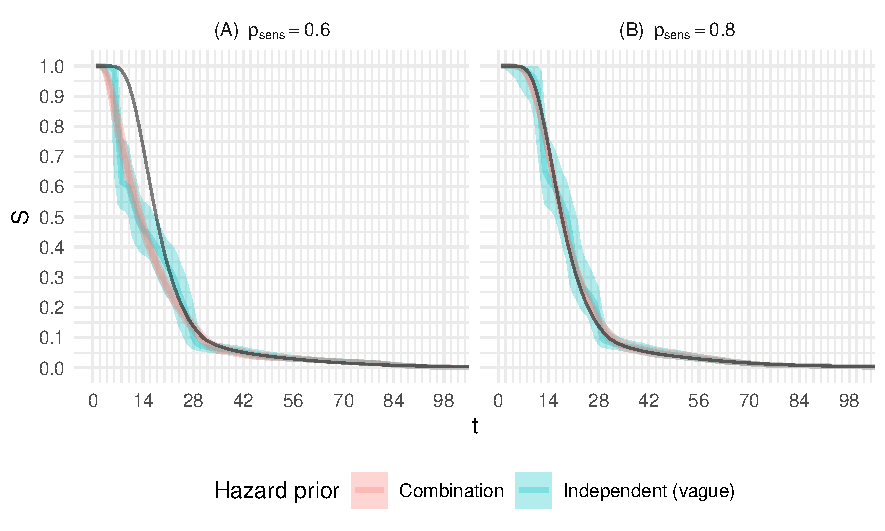
\includegraphics[width=\textwidth]{cis-imperfect-testing/sim-constant-sensitivity}
  \todo[inline]{Add simulation study figures}
  \caption[Simulation study results with constant test sensitivity]{%
    Posterior (median and 95\% credible interval) of the survival time for the simulation study with a correctly specified test sensitivity.
    True survival time shown in black.
  }
  \label{imperf-test:fig:constant-test-sensitivity}
\end{figure}

Next, we considered the consequence of $\psens$ being misspecified and using the model combination prior, the better performing prior in the correctly specified case.
If the test sensitivity is misspecified then the survival time is biased.
If $\psensi < \psenss$, then the posterior estimate initially follows the true value but then separates (see \cref{imperf-test:fig:misspecified-test-sensitivity}(A)).
The number of episodes inferred to have truly ended by the first negative is too low, and hence the survival time is overestimated.
This effect dominates over the opposing bias of overestimating the number of undetected episodes.
The opposite occurs if $\psensi > \psenss$, although the posterior moves away from the truth earlier (see \cref{imperf-test:fig:misspecified-test-sensitivity}(C)).
\begin{figure}
  % \makebox[\textwidth][c]{
    % 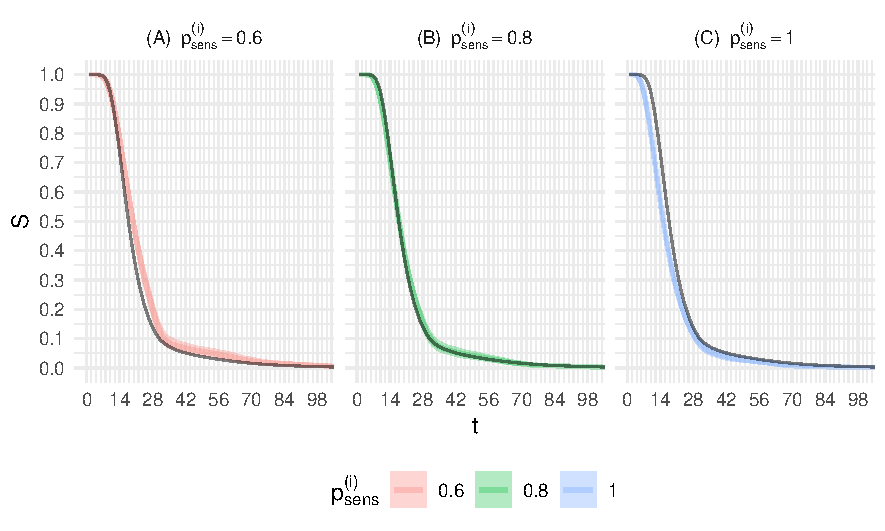
\includegraphics[width=\textwidth]{cis-imperfect-testing/sim-misspecified-sensitivity}
  \todo[inline]{Add simulation study figures}
  \caption[Simulation study results with misspecified test sensitivity]{%
    Posterior (median and 95\% credible interval) of the survival time for the simulation study with a possibly misspecified test sensitivity.
    The true survival time is shown in black.
    All results use $\psenss = 0.8$, but $\psensi$ varies, as per panel labels.
    Hence, (B) is correctly specified but (A) and (C) have misspecified $\psens$.
  }
  \label{imperf-test:fig:misspecified-test-sensitivity}
\end{figure}

The results when $\psenss = v$ are similar to $\psenss = 0.8$ (see \cref{imperf-test:fig:variable-test-sensitivity}).
This suggests that the simplified model, with constant test sensitivity, is sufficient for recovering the true survival time.
% Estimating the test sensitivity is not possible without a more complex model, as discussed in \cref{imperf-test:sec:discussion}.
Therefore, we conclude that including a varying test sensitivity is not required for adequate inference, and apply it to the real CIS data in the next section.
\begin{figure}
  % \makebox[\textwidth][c]{
    % 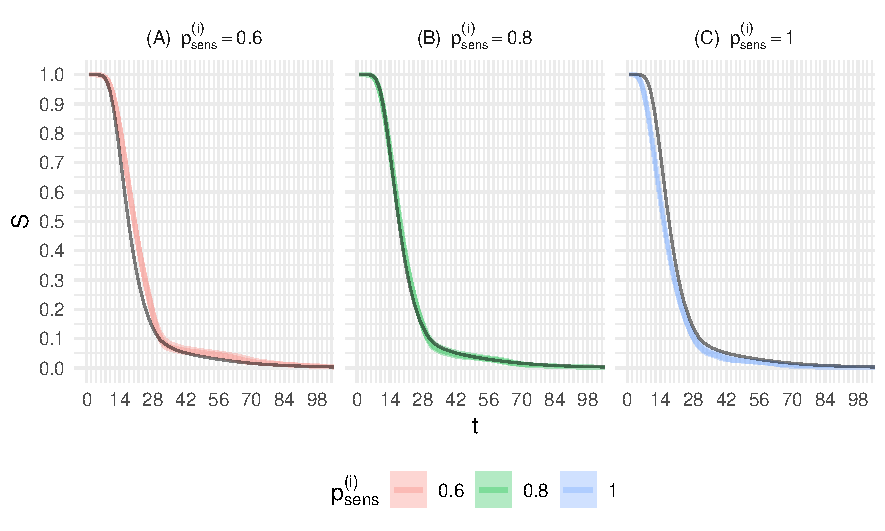
\includegraphics[width=\textwidth]{cis-imperfect-testing/sim-variable-sensitivity}
  \todo[inline]{Add simulation study figures}
  \caption[Simulation study results with varying test sensitivity]{%
    Posterior (median and 95\% credible interval) of the survival time for the simulation study with a variable test sensitivity.
    Each panel shows the results of performing inference with a different assumed value for the test sensitivity.
    The posterior estimate using a model with a constant test sensitivity of 0.8 (B) is similar to the true value (black line).
  }
  \label{imperf-test:fig:variable-test-sensitivity}
\end{figure}

\section{Application to the CIS data}

In this section we apply the approach described in this chapter to the CIS infection episode dataset.
Unlike in the simulation studies, an uninformative prior on $\ntot$ led to implausible estimates of the duration distribution.
The uninformative prior led to high posterior estimates of $\ntot$, and hence an implausibly large number of episodes with durations of less than five days.
Therefore, we used an informative prior for $\ntot$, $\ntot \sim \NBc(\mu\inform, r\inform)$ from pre-existing estimates of the total number of infections to give $\mu\inform$ and $r\inform$.
\citet{birrellRTM2} estimated the total number of infections in England over the time period we consider, with posterior mean \numprint{4136368} and standard deviation \numprint{27932}.
\todo{is there a citation for the latest RTM paper now?}
% This model gives a posterior mean of \numprint{4136368} cumulative infections in England in the time period we consider, with a posterior standard deviation of \numprint{27932}~\citePersonalComms{Paul Birrell}.
Approximating this distribution as a negative binomial and scaling the mean to the size of the CIS cohort gives the prior $\mu\inform = 25132$ and $r\inform = 22047$.

With this prior, the model produces plausible estimates of the duration distribution (see \cref{imperf-test:fig:cis-estimates}).
The estimate (blue) has more long episodes than the ATACCC-based estimate used for the prior in \cref{sec:informative-prior} (red).

The qualitative increase in long episodes is robust to the choice of prior for $\ntot$, the assumed value for $\psens$ (see \cref{imperf-test:fig:cis-sensitivity}), and the choice of prior for the hazards, $\lambda_t$.
However, the survival proportion over the first 4 weeks is sensitive to these choices.
The estimate using a test sensitivity of 0.8 and $\NBc(\mu\inform, r\inform)$ give a median survival time most similar to the ATACCC-based estimate.
\begin{figure}
  \todo[inline]{Add real data figures}
  % \centering 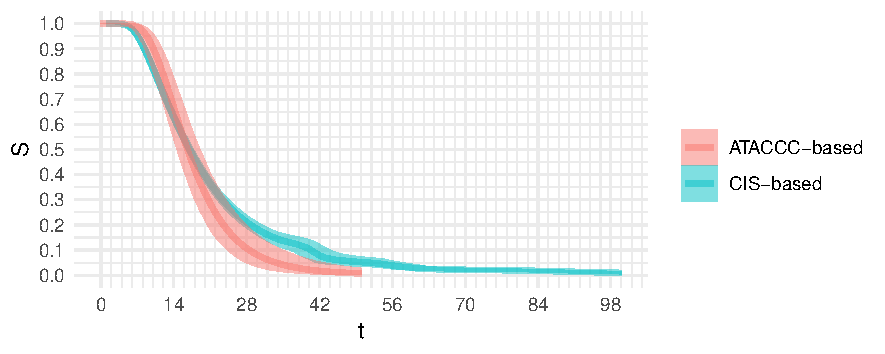
\includegraphics{cis-imperfect-testing/CIS_final}
  \caption{Duration estimates using CIS and ATACCC data}
  \label{imperf-test:fig:cis-estimates}
\end{figure}
\begin{figure}
  \vspace{-2.5cm}
  \todo[inline]{Add real data figures}
  % \makebox[\textwidth][c]{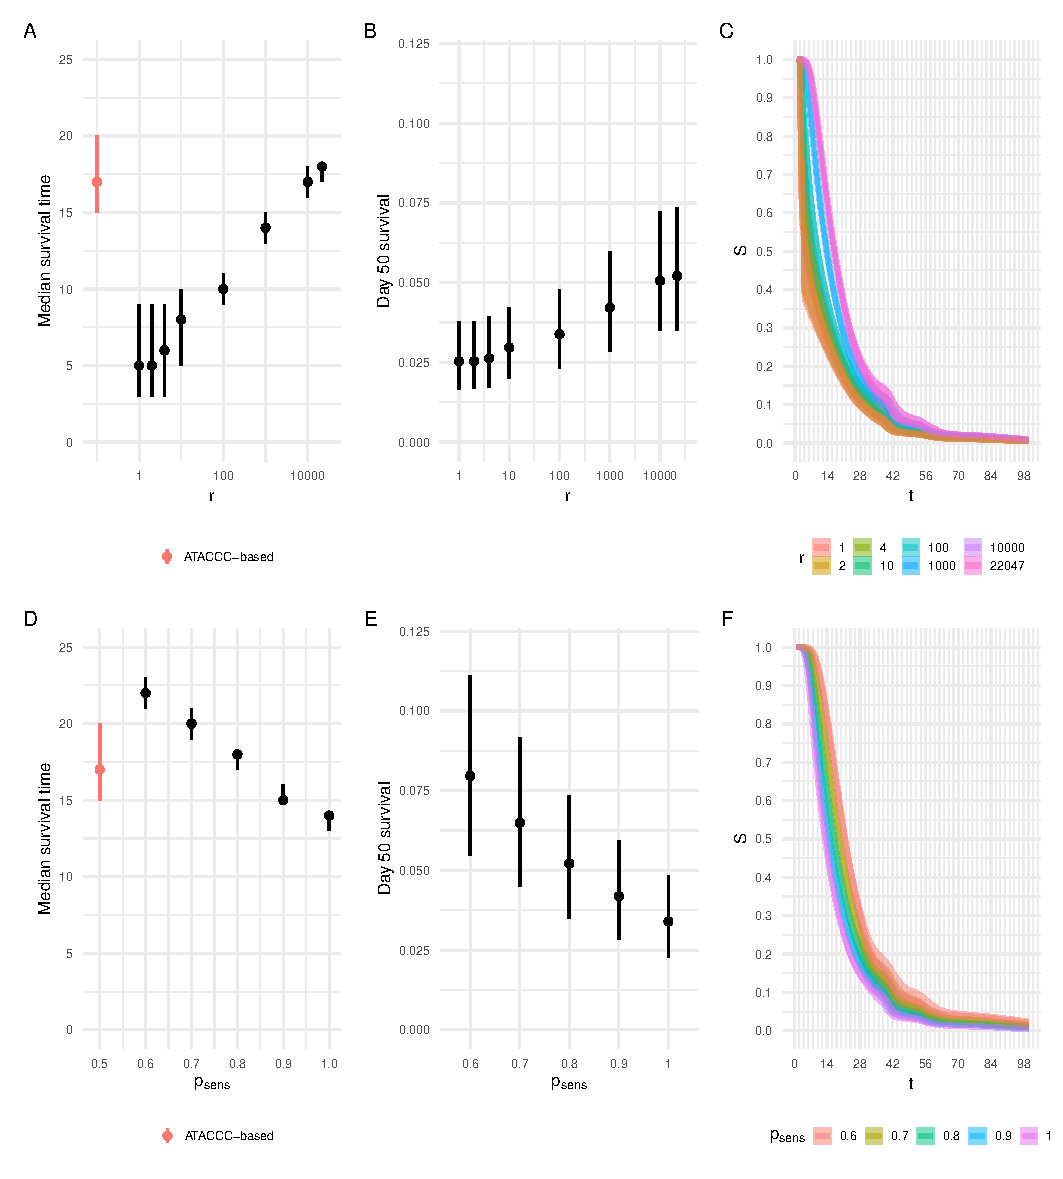
\includegraphics{cis-imperfect-testing/CIS_vary}}
  \caption{%
    (A-C) Sensitivity of CIS estimates to the value of $r$, the dispersion of the prior for $\ntot$ (a larger $r$ means a more informative prior) when $\psens = 0.8$.
    (D-F) Sensitivity of CIS estimates to the value of $\psens$ when $r = r\inform$.
    A and D: median survival time, in comparison to the ATACCC-based estimate used in the prior (shown in red).
    B and E: survival at day 50, $S_\theta(50)$.
    C and F: full survival curves out to day 100.
  }
  \label{imperf-test:fig:cis-sensitivity}
\end{figure}


The estimates are sensitive to the choice of $r$, the strength of the prior on $\ntot$.
A low value for $r$, giving a very weak, almost uninformative, prior on $\ntot$ causes its posterior estimate to be much higher than the estimate from \citet{birrellRTM2}.
When increasing the prior's strength, the posterior estimate moves towards the prior smoothly, as expected (see \cref{imperf-test:fig:ntot}).
As discussed previously, the prior information is reliable for the first 2--3 weeks, notably including the median time.
The median using $r\inform$ matched the prior's median estimate and is a principled choice because it is based directly on the prior work \citet{birrellRTM2}.
Therefore, we recommend this estimate, which has a mean survival time of 21.2 days (95\% CrI: 20.5--21.9).
\begin{figure}
  % \centering 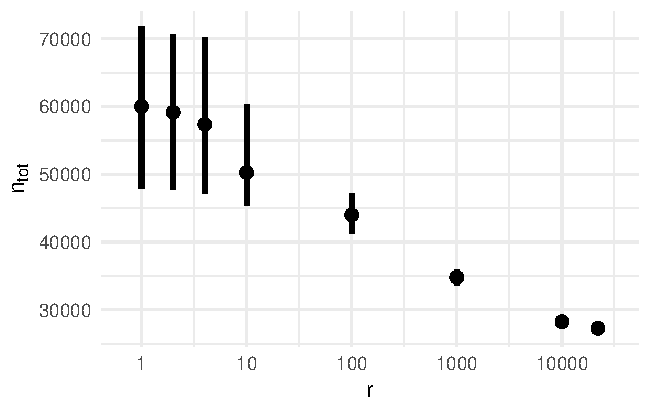
\includegraphics{cis-imperfect-testing/CIS_ntot}
  \todo[inline]{Add real data figures}
  \caption[Sensitivity of $\ntot$'s posterior to its prior.]{How the posterior estimate of $\ntot$ changes with the value of $r$ in the prior on $\ntot$.}
  \label{imperf-test:fig:ntot}
\end{figure}


\section{Discussion} \label{sec:discussion}

\todo[inline]{There's a lot of discussion points here, I've just copied these across from my thesis. I think probably too many, especially the focus on limitations; this section is about 3x longer than the standard discussion section in a JASA applications article. I'm not sure which are the interesting ones to keep and which to cut though.}

In this article, we developed a method to analyze doubly censored data with undetected events, when these undetected events occur with an arbitrary pattern in known individuals and the test sensitivity is imperfect.
We extended a previous survival analysis framework to this setting, incorporating the information on individuals with undetected events and extending the model to account for false negatives.
Our work is motivated by the desire to estimate the duration of SARS-CoV-2 infections from the CIS dataset.
The CIS was one of very few long-running, general population studies conducted during the COVID-19 pandemic, and is likely to serve as a template for studies in future pandemics.
Therefore, this work is valuable for future studies that may have similar data.

We found that an informative prior on $\ntot$, the total number of infections that occurred, is required is for the bulk of the distribution to agree with previous work.
In the simulation study, the uninformative prior on $\ntot$ performed well, even when the test sensitivity was misspecified.
A possible explanation is that the true changes in the test sensitivity is significantly different to the simulated test sensitivity
In particular, the test sensitivity for long episodes may become much lower than 50\%.
This allows many more episodes to be missed than the model assumes, and hence a higher $\ntot$ is required to explain the data.
Furthermore, it violates assumptions made in \cref{sec:false-negatives}; this is similar to when the simulating using a too low test sensitivity.
Violating these assumptions would lead to unpredictable inference results, perhaps those seen here.
Alternative study designs could be useful in providing more information on the duration of infection episodes.
For example, following up the first positive test for an infection episode with more frequent testing would allow the episode's end to be more accurately determined.

We assumed a prior of constant incidence and that the time infection episodes begin is independent between individuals.
Prevalence in the CIS data was approximately constant over the period of interest.
A sensitivity analysis, where an epidemic in exponential growth or decline was simulated (not shown), showed minimal impact on survival estimates.
An incorrect assumption of constant incidence can lead to biased estimates~\autocite{degruttolaAnalysis}.
Therefore, the assumption could be important in other contexts, especially if the incidence is changing rapidly.


The derivation in \cref{sec:inference} relied on an assumption that $O(j)$ and $O(j')$ occur independently for $j \neq j'$.
This is not the case, as immunity means that an individual previously infected is less likely to be infected in the future.
Additionally, the same individual cannot have multiple detected concurrent infections, due to the way that the episodes dataset is constructed; this limits certain combinations from occurring.
In practice, this means that $n_k > 1$ cannot occur.
The simulation study violated this assumption to a large extent: each individual could only have one infection.
Despite this, the method performed well when $\psens = 1$, recovering the true survival function.
Therefore, it is unlikely that this assumption matters, possibly due to the large number of individuals without detected episodes.
Further work could explore different assumptions, \eg a ``full immunity'' assumption meaning each individual has zero or one episode in the period.

Ideally, the test sensitivity would be estimated from the data.
However, this would require incorporating time-varying test sensitivity into the likelihood.
If the current model, with a constant $\psens$, is used then the estimate of $\psens$ would be heavily informed be intermittent negatives (the first, constant term in \cref{imperf-test:eq:pia-prime}).
These negatives will, in general, be further from the end of an episode than a randomly selected test.
Therefore, considering the viral dynamics from \cref{E-ATACCC}, the viral load will be higher and false negatives rarer.

Estimating the test sensitivity excluding intermittent negatives is not possible because \cref{imperf-test:eq:pia-prime-constant,imperf-test:eq:pit-prime} are both monotonically decreasing in $\psens$; therefore, the likelihood always favours $\psens = 0$ (\ie no true positives).
This aligns with the situation with singly interval censored, untruncated data, when stopping at the first observed time of the terminating event (which may be misclassified) means that the test sensitivity cannot be estimated~\citep[e.g.]{titmanMisclassify}.

Estimating a time-varying $\psens$ with $S_\theta$ jointly may cause identifiability issues.
Previous studies have avoided issues by including external information (such as a prior giving the magnitude) on $\psens$, or test results from later follow-up~\citep[and references therein]{piresIntervalMisclassify}.
However, these studies use a constant $\psens$.
Whether these methods are sufficient for the model to be identifiable with a time-varying $\psens$ needs further investigation.
A simple parametric form of the test sensitivity, such as that proposed by \citet{brownBayesian}, may be sufficient to allow identifiability.
In any case, the likelihood, especially $p_{iu}'$, would be substantially complicated by such an addition which may greatly increase the computational cost of inference.

We provide a flexible simulation and inference framework for this type of analysis.
This framework could be used to simulate alternate study designs.
The design of CIS was created on a very short timescale in March 2020, in response to the pandemic's rapid spread.
Therefore, it is likely that there are more efficient designs.
These could be more cost-effective.
Improved cost-effectiveness could allow more rapid response to potential pandemics because the threshold for policymakers to approve the study would be lower.
A long-term, preparatory effort to develop a more efficient design in preparation for a future pandemic would be worthwhile.

Other useful preparatory work would be developing reasonable priors.
These could be based on seasonal viruses that are of the same family as those likely to cause future pandemics.
For example, seasonal influenzas and coronaviruses.
These would allow analyses such as those performed in these chapters to be performed more rapidly in a future pandemic scenario.

\bibliographystyle{agsm}

\bibliography{references}


\appendix

\section{Derivations}

\begin{align}
p(\vec{\theta} \mid \na)
&\propto p(\vec{\theta}) p(\na \mid \vec{\theta}) \\
&= p(\vec\theta) \sum_{\ntot= \ndet}^{\infty} p(\ntot, \na \mid \vec{\theta}) \\
&= p(\vec{\theta}) \sum_{\ntot=\ndet}^\infty p(\ntot \mid \vec{\theta}) p(\na \mid \ntot, \vec{\theta}) \\
&= p(\vec{\theta}) \sum_{\ntot=\ndet}^\infty p(\ntot \mid \vec{\theta}) \frac{\ntot!}{(\ntot - \ndet)!} \pnodet^{\ntot - \ndet} \prod_{k \in \set{D}} p_k &\text{by \cref{perf-test:eq:multinomial}} \\
&= p(\vec{\theta}) \left( \prod_{k \in \set{D}} p_k \right) \left( \sum_{\ntot=\ndet}^\infty p(\ntot \mid \vec{\theta}) \frac{\ntot!}{(\ntot - \ndet)!} \pnodet^{\ntot - \ndet} \right).
\intertext{For convenience, define the summation term as:}
\eta &= 
\sum_{\ntot=\ndet}^\infty p(\ntot \mid \vec{\theta}) \frac{\ntot!}{(\ntot - \ndet)!} \pnodet^{\ntot - \ndet}.
\end{align}

\subsection{Expression for $\eta$}


We derive an analytical solution to $\eta$ (defined in \cref{perf-test:eq:eta}).
We assume the prior $\ntot \dist \NBc(\mu, r)$, and that it is independent of $\vec{\theta}$, the parameters of the survival distribution.
Therefore, $p(\ntot \mid \vec{\theta}) = p(\ntot)$.
This assumption makes $\eta$ analytically tractable, allowing computationally feasible inference.

Putting a negative binomial prior on $\ntot$ is equivalent to the following gamma-Poisson composite; its use simplifies the derivation.
\begin{align}
\ntot \mid \lambda &\dist \Poi(\lambda) \\
\lambda &\dist \GamDist(a, b)
\end{align}
where $b = r / \mu$ and $a = r$.
Hence:
\begin{align}
\eta
&= \int \sum_{\ntot=\ndet}^\infty \frac{\ntot!}{(\ntot-\ndet)!} \pnodet^{\ntot-\ndet} p(\ntot \mid \lambda) p(\lambda) d\lambda &\text{$\lambda$ explicit}\\
&= \int \sum_{\ntot=\ndet}^\infty \frac{\ntot!}{(\ntot-\ndet)!} \pnodet^{\ntot-\ndet} \frac{\lambda^{\ntot} e^{-\lambda}}{\ntot!} p(\lambda) d\lambda &\ntot \dist \Poi\\
%&= \int \sum_{\ntot=\ndet}^\infty \frac{1}{(\ntot-\ndet)!} \pnodet^{\ntot-\ndet} \lambda^{\ntot-\ndet} \lambda^{\ndet} e^{-\lambda} p(\lambda) d\lambda \\
&= \int \lambda^{\ndet} e^{-\lambda} p(\lambda) \sum_{\nnodet=0}^\infty \frac{(\pnodet \lambda)^{\nnodet}}{\nnodet!} d\lambda &\nnodet = \ntot-\ndet\\
&= \int \lambda^{\ndet} e^{-\lambda} p(\lambda) e^{\lambda \pnodet} d\lambda &\text{Maclaurin series of $e$} \\
&= \int \lambda^{\ndet} e^{-\lambda(1 - \pnodet)} \frac{b^a}{\Gamma(a)} \lambda^{a-1} e^{-b\lambda} d\lambda &\lambda \dist \GamDist\\
&= \int \frac{b^a}{\Gamma(a)} \lambda^{a+\ndet-1} e^{-(b+1-\pnodet)\lambda} d\lambda \\
&= \frac{b^a}{\Gamma(a)} \frac{\Gamma(a+\ndet)}{(b+1-\pnodet)^{a+\ndet}} &\text{Gamma pdf}\\
&\propto (b+1-\pnodet)^{-(a+\ndet)} &\text{only $p_u$ depends on $\theta$}\\
&= (r/\mu + 1 - \pnodet)^{-(r+\ndet)} &\text{sub in $\mu$ and $r$}\\
&\propto(r + \mu (1- \pnodet))^{-(r+\ndet)}.
\end{align}

Substituting this into \cref{perf-test:eq:posterior1} gives:
\begin{align}
p(\vec{\theta} \mid \na)
&\propto p(\vec{\theta}) \left( \prod_{i \in \set{D}} p_k \right) (r + \mu (1- \pnodet))^{-(r+\ndet)}.
\end{align}


Omitting the conditioning
If $i_j = i_k$ then the event $O_j = \vec{\nu}_k$ occurs if and only if the episode starts in the interval $[l^{(b)}_k, r^{(b)}_k]$ and ends in the interval $[l^{(e)}_k, r^{(e)}_k]$.
 on $\vec{\theta}$ and $i_j = i_k$, this gives:
\begin{align}
p_{ik}
=& \prob \left( l_k^{(b)} \leq B_{j} \leq r_k^{(b)}, l_k^{(e)} \leq E_{j} \leq r_k^{(e)} \right) \\
=& \prob \left( l_k^{(e)} \leq E_{j} \leq r_k^{(e)} \mid l_k^{(b)} \leq B_{j} \leq r_k^{(b)} \right) \times\prob \left( l_k^{(b)} \leq B_{j} \leq r_k^{(b)} \right) \\
=& \sum_{b = l_k^{(b)}}^{r_k^{(b)}} \prob \left( l_k^{(e)} \leq E_{j} \leq r_k^{(e)} \mid B_{j} = b \right) \prob \left(B_{j} = b \right) \\
=& \sum_{b = l_k^{(b)}}^{r_k^{(b)}} \prob \left( l_k^{(e)} - b + 1 \leq D_{j} \leq r_k^{(e)} - b + 1 \right) \prob \left(B_{j} = b \right) &\text{by def of $D_{j}$} \\
=& \sum_{b = l_k^{(b)}}^{r_k^{(b)}} \left( S_{\vec{\theta}}(l_k^{(e)} - b + 1) - S_{\vec{\theta}}(r_k^{(e)} - b + 2) \right) \prob \left(B_{j} = b \right) &\text{by def of $S_{\vec{\theta}}$} \\
\propto& \sum_{b = l_k^{(b)}}^{r_k^{(b)}} \left( S_{\vec{\theta}}(l_k^{(e)} - b + 1) - S_{\vec{\theta}}(r_k^{(e)} - b + 2) \right)
\label{perf-test:eq:pia}
\end{align}
under the assumption of uniform probability of infection time.
This is the standard form of the likelihood for doubly interval censored data without truncation~\citep[e.g.][]{sunEmpirical}.


\bigskip
\begin{center}
{\large\bf SUPPLEMENTARY MATERIAL}
\end{center}

\begin{description}

\item[Title:] Brief description. (file type)

\item[R-package for  MYNEW routine:] R-package MYNEW containing code to perform the diagnostic methods described in the article. The package also contains all datasets used as examples in the article. (GNU zipped tar file)

\item[HIV data set:] Data set used in the illustration of MYNEW method in Section~ 3.2. (.txt file)

\end{description}
\end{document}